\chapter{Frequency Response}

\begin{figure}[H]
  \centering
  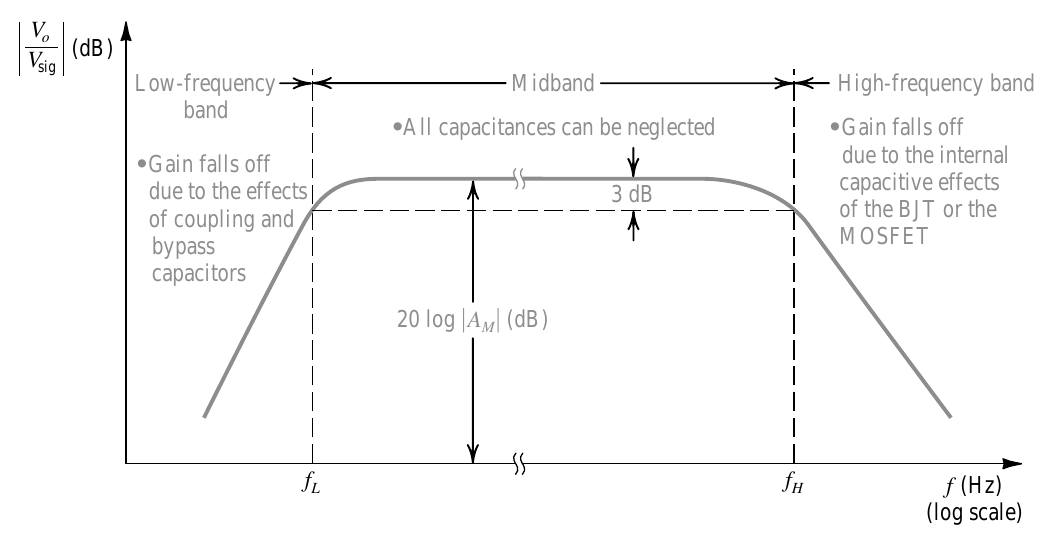
\includegraphics[width=0.6\linewidth]{figures/Frequency-Response}
  \caption{Sketch of the gain of amplifier versus frequency}
  \label{fig:}
\end{figure}

\section{Low-Frequency}

\subsection{Common-Source Amplifier}

\begin{figure}[H]
  \centering
  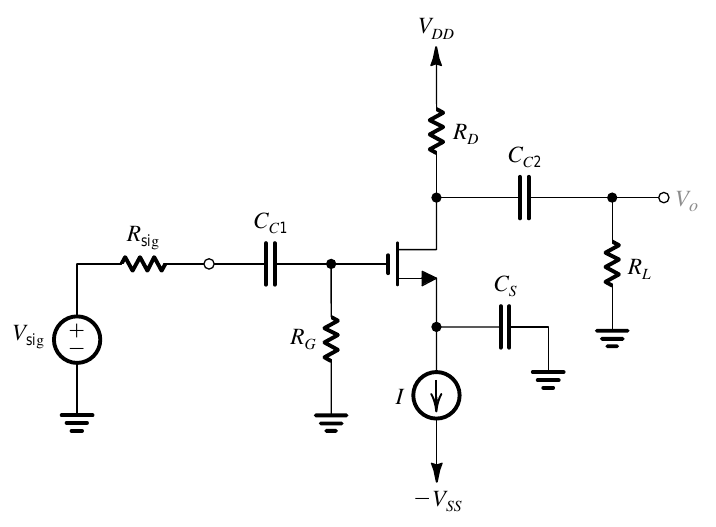
\includegraphics[width=0.6\linewidth]{figures/Frequency-Response-CS}
  \label{fig:}
\end{figure}

\begin{equation*}
  \begin{aligned}
    A_M = - \dfrac{R_G}{R_G + R_{sig}} \left[ g_m \left( R_D \parallel R_L \right) \right]  
  \end{aligned}
\end{equation*}

\begin{equation*}
  \begin{aligned}
    \omega_{p1} &= \dfrac{1}{C_{C1} \left( R_G + R_{sig} \right)} \\
    \omega_{p2} &= \dfrac{g_m}{C_S} \\
    \omega_{p3} &= \dfrac{1}{C_{C2} \left( R_D + R_L \right)} 
  \end{aligned}
\end{equation*}

\begin{equation*}
  \begin{aligned}
    \dfrac{V_o}{V_{sig}} &= A_M \left( \dfrac{s}{s + \omega_{p1}}  \right) \left( \dfrac{s}{s + \omega_{p2}}  \right) \left( \dfrac{s}{s + \omega_{p3}}  \right) 
  \end{aligned}
\end{equation*}

\begin{figure}[H]
  \centering
  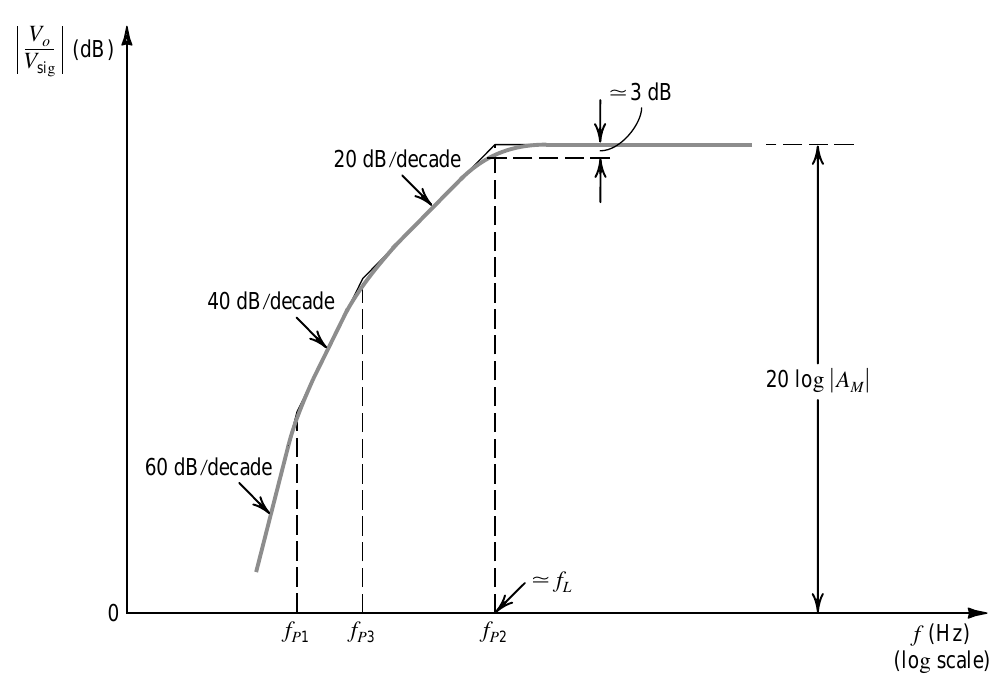
\includegraphics[width=0.6\linewidth]{figures/Frequency-Response-CS-freq}
  \label{fig:}
\end{figure}

\begin{equation*}
  \begin{aligned}
    f_L \approx f_{p2} = \dfrac{\omega_{p2}}{2 \pi} = \dfrac{1}{2 \pi \left( C_s / g_m  \right)} 
  \end{aligned}
\end{equation*}

\subsection{Common-Emitter Amplifier}

\begin{figure}[H]
  \centering
  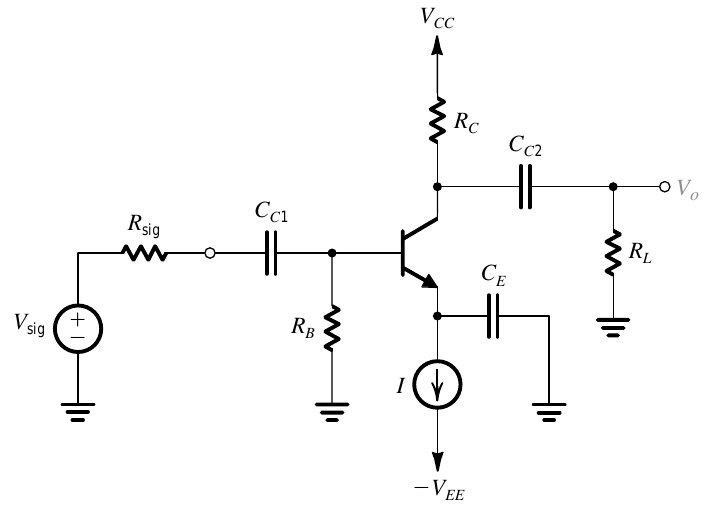
\includegraphics[width=0.4\linewidth]{figures/Frequency-Response-CE}
  \label{fig:}
\end{figure}

\begin{equation*}
  \begin{aligned}
    A_M = - \dfrac{\left( R_B \parallel r_{\pi} \right)}{\left( R_B \parallel r_{\pi} \right) R_{sig} } g_m \left( R_C \parallel R_L \right) 
  \end{aligned}
\end{equation*}

\begin{equation*}
  \begin{aligned}
    \omega_{p1} &= \dfrac{1}{C_{C1} \left[ \left( R_B \parallel r_{\pi} \right) + R_{sig} \right]} \\
    \omega_{p2} &= \dfrac{1}{C_E \left[ r_e + \dfrac{R_B \parallel R_{sig}}{\beta + 1}  \right]} \\
    \omega_{p3} &= \dfrac{1}{C_{C2} \left( R_C + R_L \right)} 
  \end{aligned}
\end{equation*}

\begin{figure}[H]
  \centering
  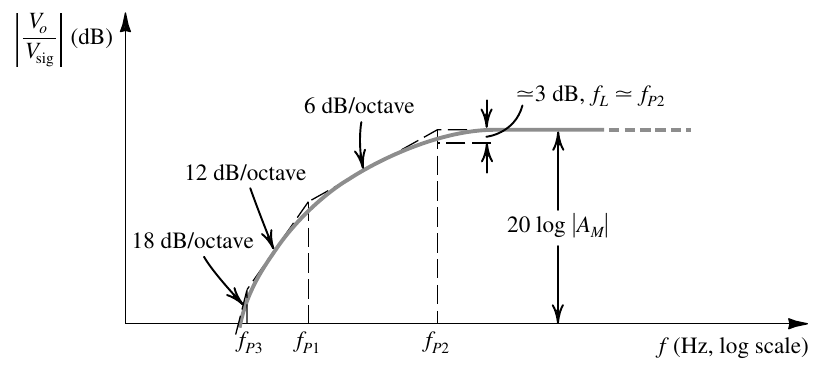
\includegraphics[width=0.5\linewidth]{figures/Frequency-Response-CE-freq}
  \label{fig:}
\end{figure}

\begin{equation*}
  \begin{aligned}
    f_L \approx f_{p2}
  \end{aligned}
\end{equation*}

\section{High-Frequency}

\subsection{Unity-Gain Frequency}

\subsubsection{MOSFET}

\begin{figure}[H]
  \centering
  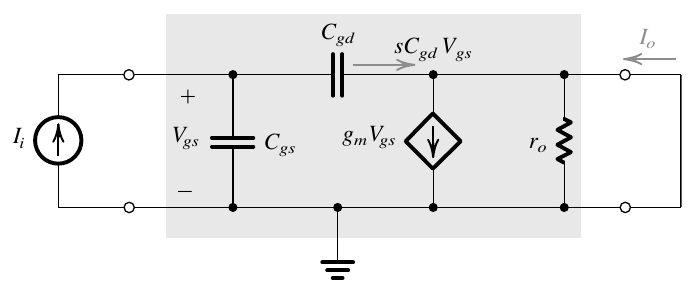
\includegraphics[width=0.5\linewidth]{figures/Frequency-Response-UG-MOS}
  \label{fig:}
\end{figure}

\begin{equation*}
  \begin{aligned}
    \dfrac{I_o}{I_i} = \dfrac{g_m}{s \left( C_{gs} + C_{gd} \right)}  \quad\quad \omega_T = \dfrac{g_m}{\left( C_{gs} + C_{gd} \right)} \quad\quad f_T = \dfrac{g_m}{2 \pi \left( C_{gs} + C_{gd} \right)} 
  \end{aligned}
\end{equation*}

\subsubsection{BJT}

\begin{figure}[H]
  \centering
  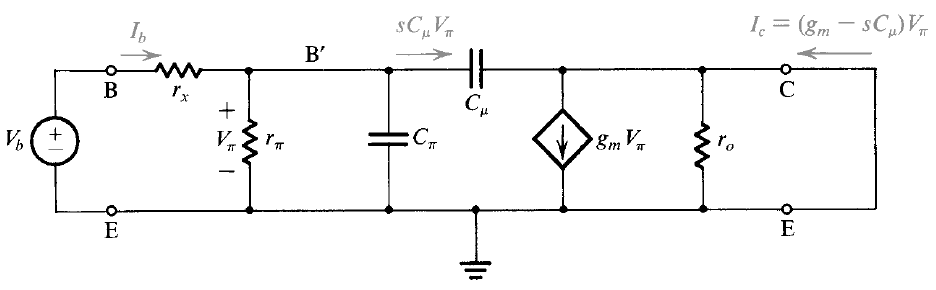
\includegraphics[width=0.7\linewidth]{figures/Frequency-Response-UG-BJT}
  \label{fig:}
\end{figure}

\begin{equation*}
  \begin{aligned}
    \dfrac{I_c}{I_b} = \dfrac{g_m r_{\pi}}{1 + s \left( C_{\pi} + C_{\mu} \right) r_{\pi}} = \dfrac{\beta_0}{1 + s \left( C_{\pi} + C_{\mu} \right) r_{\pi}} \quad\quad \omega_{\beta} = \dfrac{1}{\left( C_{\pi} + C_{\mu} \right) r_{\pi}} \quad\quad \omega_T = \beta_0 \omega_{\beta} = \dfrac{g_m}{C_{\pi} + C_{\mu}}     
  \end{aligned}
\end{equation*}

\subsection{Common-Source Amplifier}

\begin{figure}[H]
  \centering
  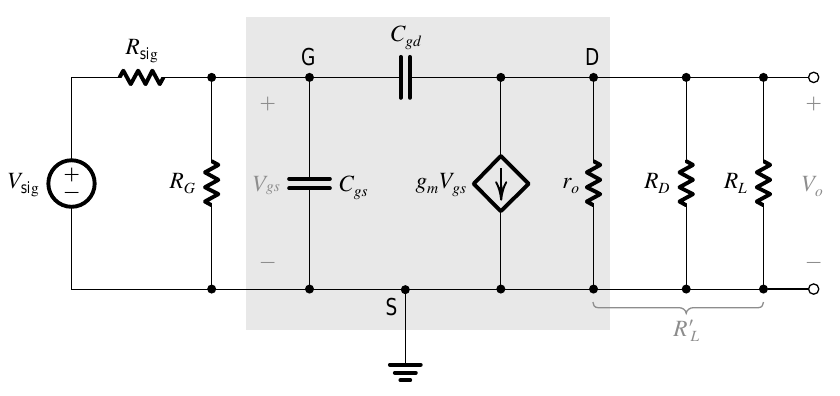
\includegraphics[width=0.9\linewidth]{figures/Frequency-Response-CS-High-1}
  \label{fig:}
\end{figure}

\begin{figure}[H]
  \centering
  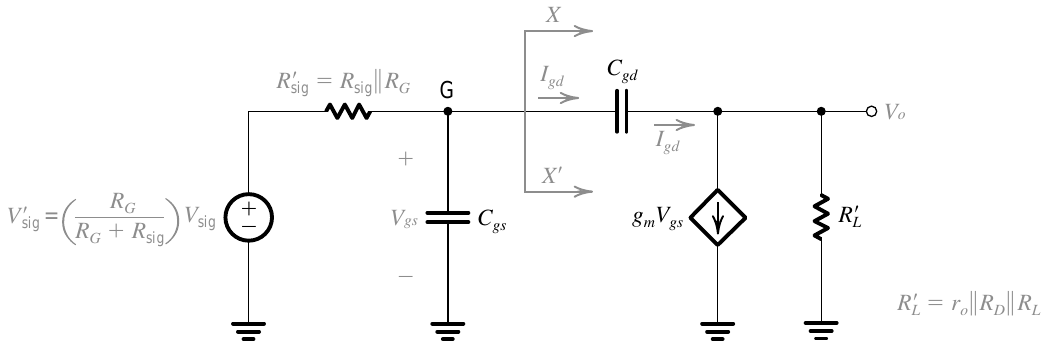
\includegraphics[width=0.9\linewidth]{figures/Frequency-Response-CS-High-2}
  \label{fig:}
\end{figure}

\begin{figure}[H]
  \centering
  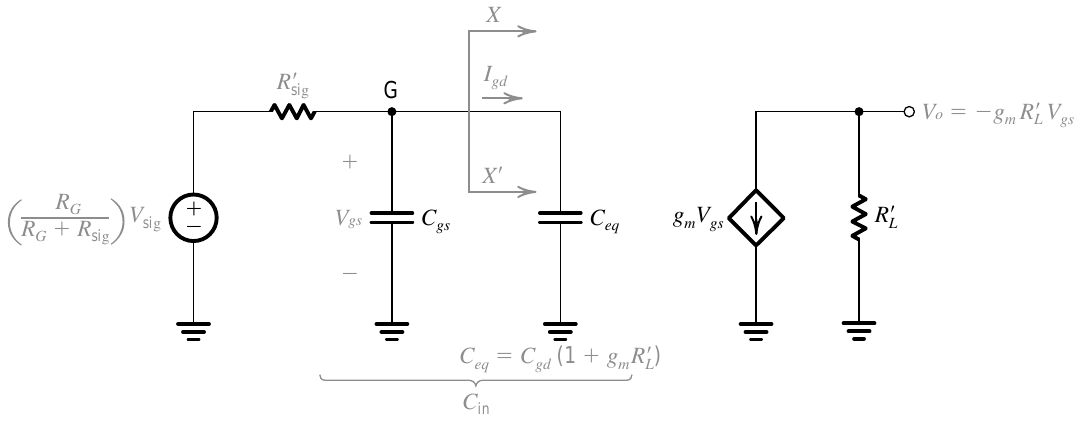
\includegraphics[width=\linewidth]{figures/Frequency-Response-CS-High-3}
  \label{fig:}
\end{figure}

\begin{equation*}
  \begin{aligned}
    \omega_H = \dfrac{1}{C_{in} R_{sig}'} \quad\quad A_M = - \dfrac{R_G}{R_G + R_{sig}} g_m R_L' \quad\quad f_H = \dfrac{\omega_H}{2 \pi} = \dfrac{1}{2 \pi C_{in} R_{sig}'}   
  \end{aligned}
\end{equation*}

\subsection{Common-Emitter Amplifier}

\begin{figure}[H]
  \centering
  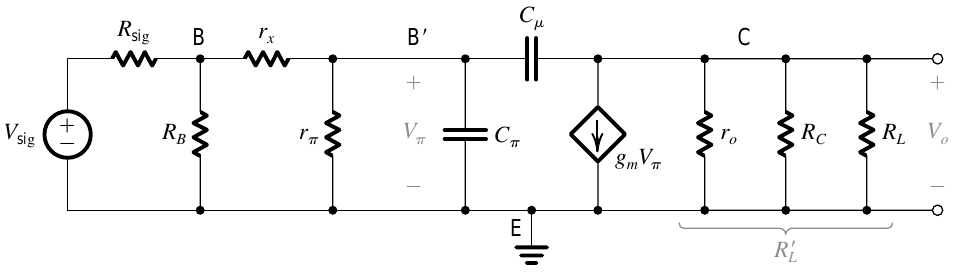
\includegraphics[width=0.9\linewidth]{figures/Frequency-Response-CE-High-1}
  \label{fig:}
\end{figure}

\begin{figure}[H]
  \centering
  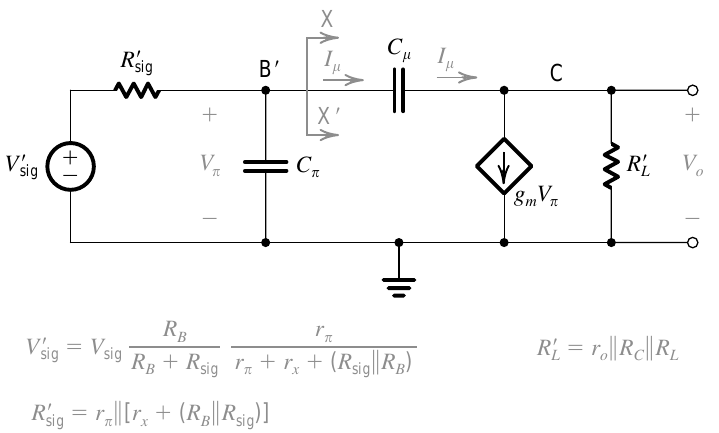
\includegraphics[width=0.8\linewidth]{figures/Frequency-Response-CE-High-2}
  \label{fig:}
\end{figure}

\begin{figure}[H]
  \centering
  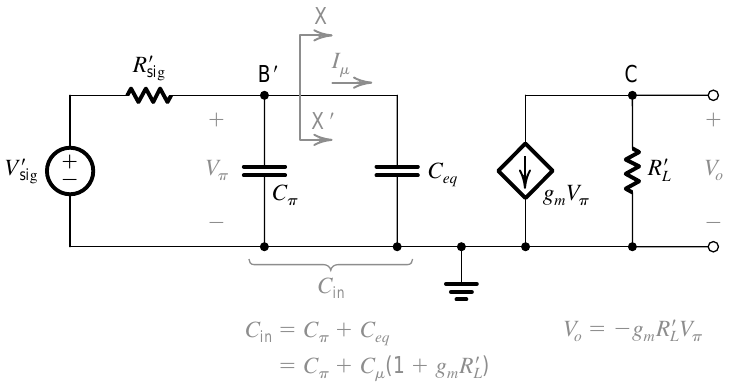
\includegraphics[width=0.8\linewidth]{figures/Frequency-Response-CE-High-3}
  \label{fig:}
\end{figure}

\begin{equation*}
  \begin{aligned}
    A_M = - \dfrac{R_B}{R_B + R_{sig}} \dfrac{r_{\pi}}{r_{\pi} + r_x + \left( R_{sig} \parallel R_B \right)} \left( g_m R_L' \right) \quad\quad f_H = \dfrac{\omega_H}{2 \pi} = \dfrac{1}{2 \pi C_{in} R_{sig}'}   
  \end{aligned}
\end{equation*}

%%% Local Variables:
%%% mode: latex
%%% TeX-master: "Analogue_Electronics"
%%% End:
